\section{Evaluation}
\label{sec:evaluation}

The evaluation consists of four parts:

\begin{itemize}
\item Application profiles (\autoref{fig:all-profiles})
\item Online Profiling (\autoref{fig:online-profiling-comparison},
  \autoref{fig:parallel}, \autoref{fig:trigger})
\item Runtime Adaptation (\autoref{fig:all-runtime})
\item Multi-task Scheduling (\autoref{fig:multitask})
\end{itemize}

\subsection{Application Profiles}
\label{sec:application-profiles}

Our system learned the application profiles for all three applications (shown in
\autoref{fig:all-profiles}). From these profiles, we make the following three
observations:

\para{Optimal strategy is achieved with multiple dimensions.} In each profile,
in addition to the Pareto-optimal strategies, we show the performance if only
one dimension is tuned. As show in the figure, they almost always lead to a
sub-optimal performance.

\para{Different dimensions have different impact for the same application.}
For pedestrian detection, tuning resolution leads to a quicker degradation in
comparison to tuning frame rate.

\para{The same dimension has different impact for different applications.}
If we compare two video analytics applications, pedestrian detection and
augmented reality, we see how tuning each dimension affects the performance
differently.

\begin{figure*}
  \centering
  \begin{subfigure}[t]{0.33\textwidth}
    \centering
    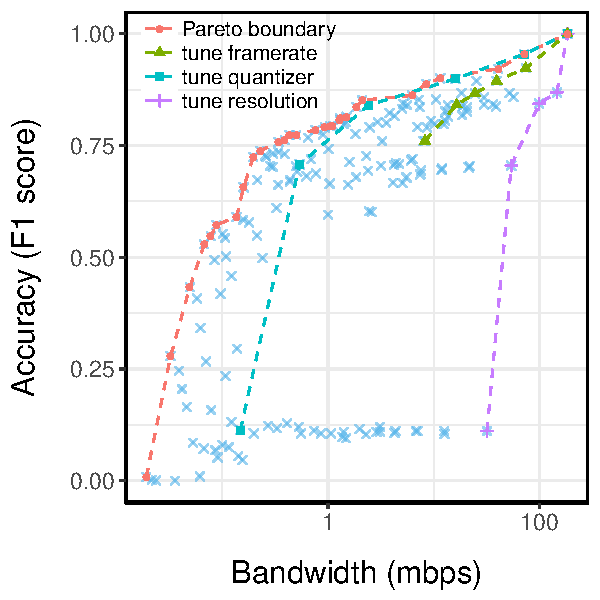
\includegraphics[width=\textwidth]{figures/ped-profile.pdf}
    \caption{Pedestrian Detection}
    \label{fig:pd-profile}
  \end{subfigure}
  ~
  \begin{subfigure}[t]{0.33\textwidth}
    \centering
    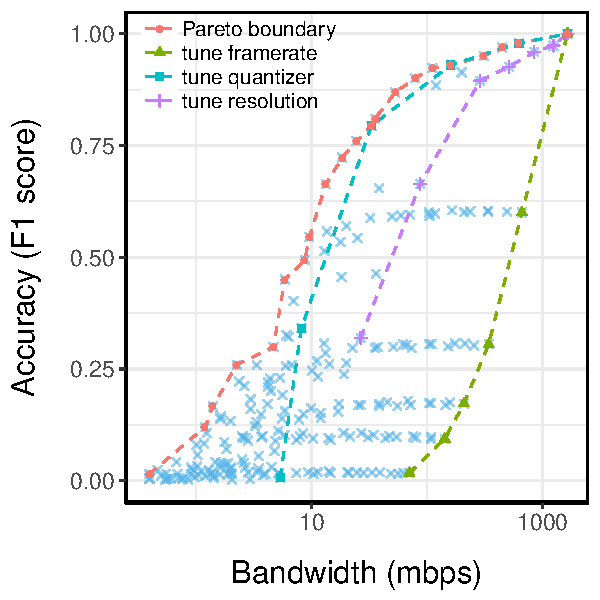
\includegraphics[width=\textwidth]{figures/darknet-profile.pdf}
    \caption{Augmented Reality}
    \label{fig:ar-profile}
  \end{subfigure}
  ~
  \begin{subfigure}[t]{0.33\textwidth}
    \centering
    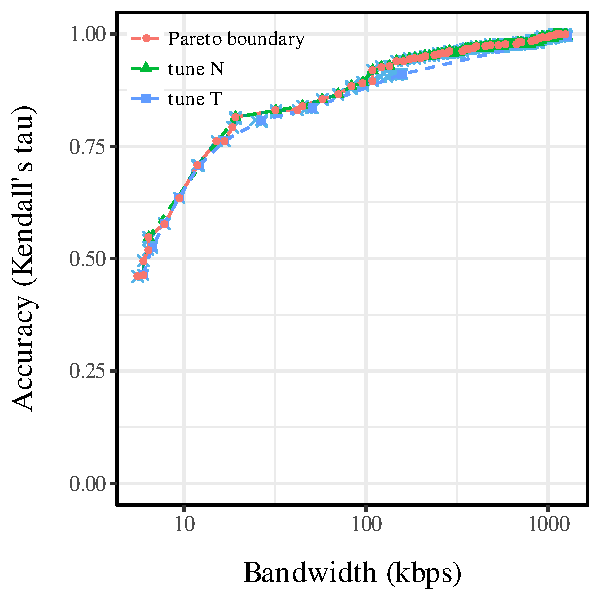
\includegraphics[width=\textwidth]{figures/topk-profile.pdf}
    \caption{Top-k}
    \label{fig:tk-profile}
  \end{subfigure}
  \caption{Application profiles.}
  \label{fig:all-profiles}
\end{figure*}

\subsection{Efficient Online Profiling}
\label{sec:online-profiling}

First, we validate the necessity for online profiling. We compare two adaptation
scheme: one with the offline learned profile; the other enabled with online
profiling. \autoref{fig:online-profiling-comparison} shows the performance
difference. Initially, both schemes work similarly. Overtime, when the data
distribution changes, the offline-learned profile doesn't match with the newly
generated data, leading to accuracy deterioration. System enabled with online
profiling is able to track the data and offers high accuracy.

\begin{figure}
  \centering
  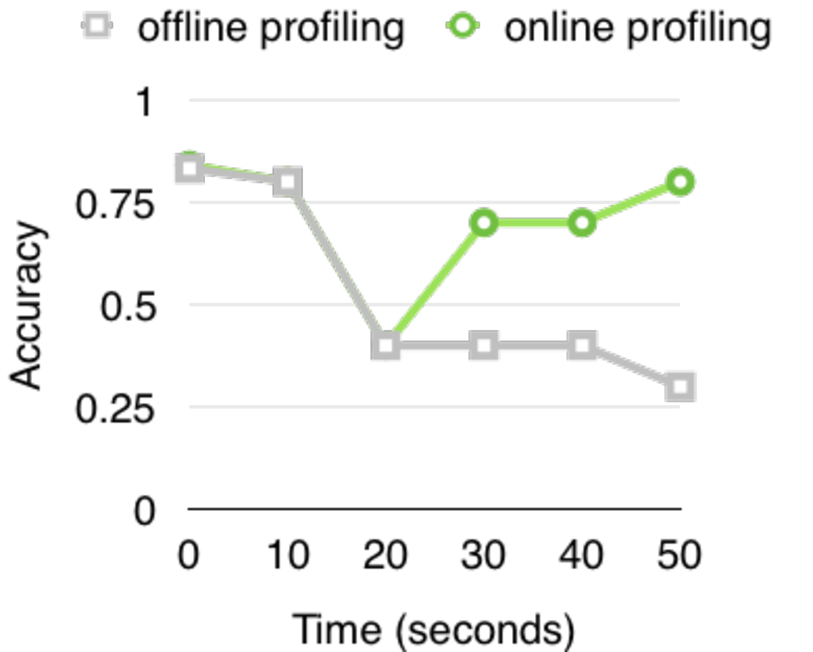
\includegraphics[width=\columnwidth]{figures/offline-online-profiling.pdf}
  \caption{The case for online profiling}
  \label{fig:online-profiling-comparison}
\end{figure}

While online profiling is beneficial, doing it naively faces the combinatorial
space search. This is different from the offline profiling that doesn't have
much time or resource constrain.

We evaluate our proposed solutions regarding the efficiency.

\para{Degradation-aware parallel profiling:} In the offline learned profile, we
have the measured time required to run for each configuration. Our parallel
profiling takes the measurements as input and generates a parallel profiling
schedule: Compare strategies for profiling.  \autoref{fig:parallel} shows our
profiling scheduling in comparison with a naive scheduler.

\begin{figure}
  \centering
  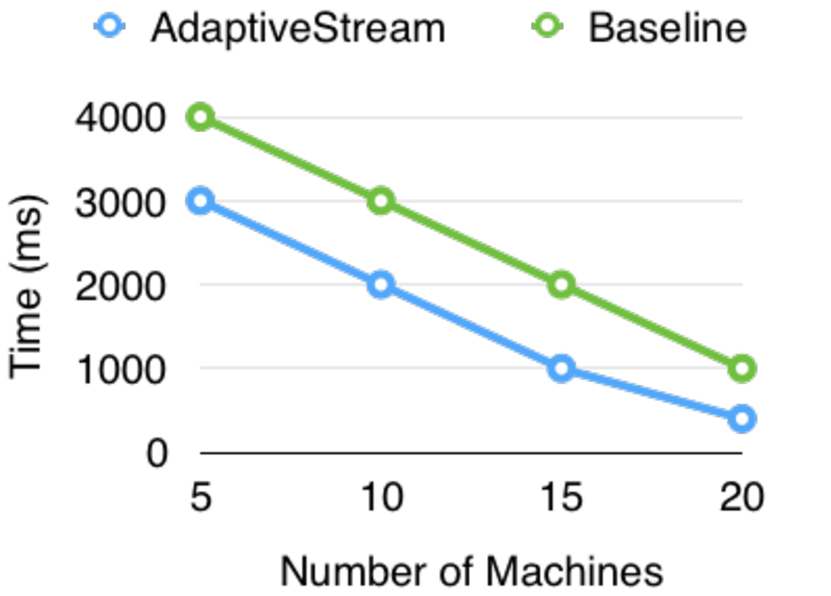
\includegraphics[width=\columnwidth]{figures/parallel-placeholder.pdf}
  \caption{Degradation-aware parallel scheduling}
  \label{fig:parallel}
\end{figure}

\para{Trigger-based profiling:} Only start the profiling when there is
substantial difference. \autoref{fig:trigger} shows the savings in trigger-based
profiling.

\begin{figure}
  \centering
  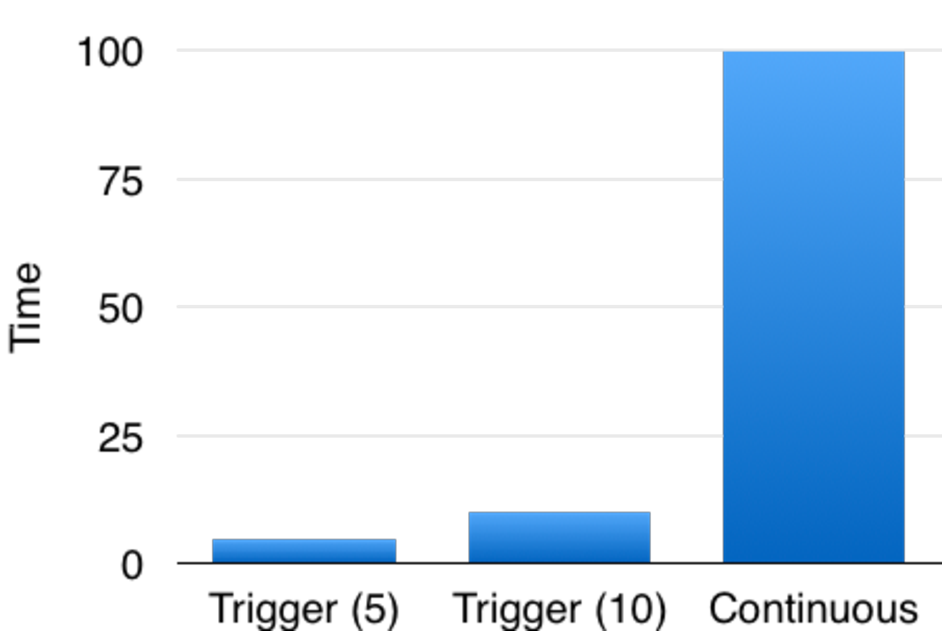
\includegraphics[width=\columnwidth]{figures/trigger.pdf}
  \caption{Trigger-based profiling}
  \label{fig:trigger}
\end{figure}

\subsection{Runtime Adaptation}
\label{sec:runtime-adaptation}

\begin{figure*}
  \centering
  \begin{subfigure}[t]{0.33\textwidth}
    \centering
    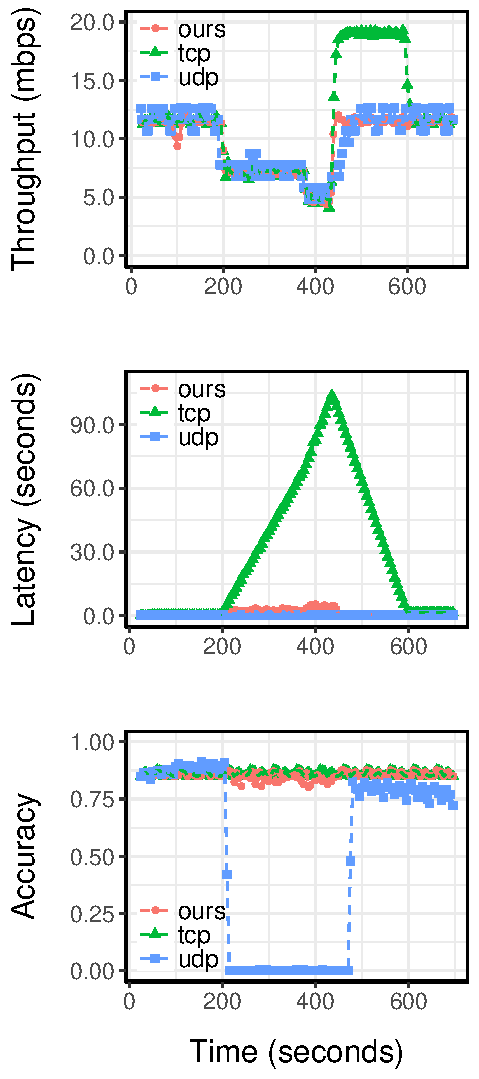
\includegraphics[width=\textwidth]{figures/ped-runtime-verticle.pdf}
    \caption{Pedestrian Detection}
    \label{fig:pd-runtime}
  \end{subfigure}
  ~
  \begin{subfigure}[t]{0.33\textwidth}
    \centering
    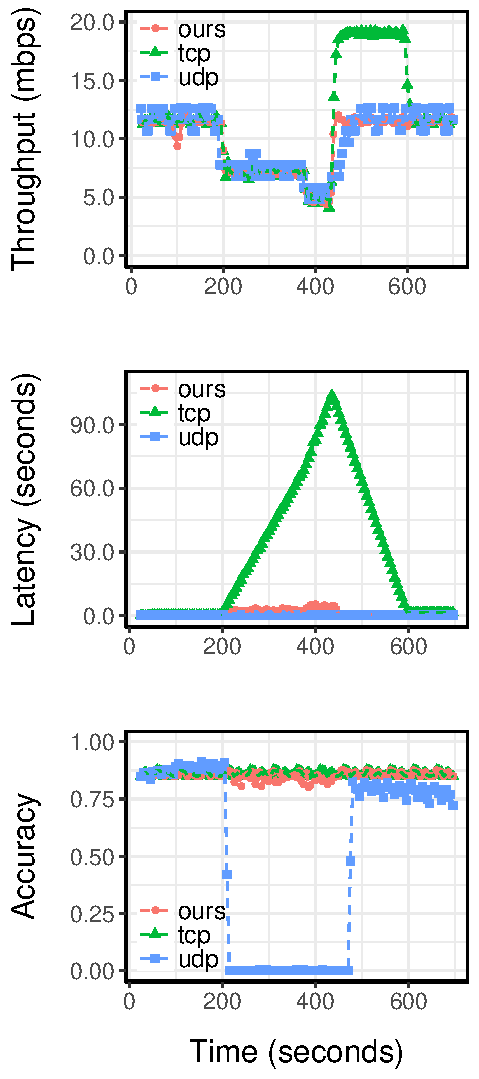
\includegraphics[width=\textwidth]{figures/ped-runtime-verticle.pdf}
    \caption{Augmented Reality}
    \label{fig:ar-runtime}
  \end{subfigure}
  ~
  \begin{subfigure}[t]{0.33\textwidth}
    \centering
    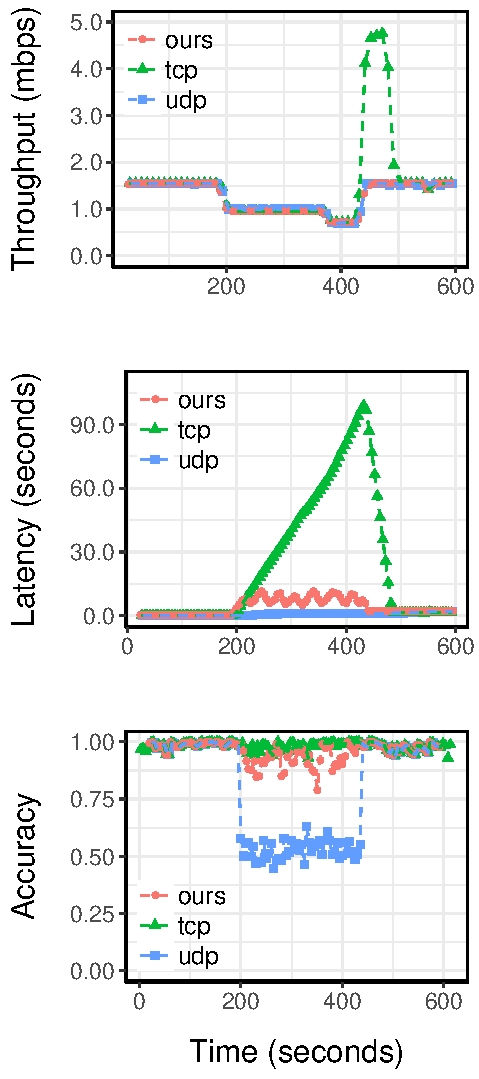
\includegraphics[width=\textwidth]{figures/topk-runtime-verticle.pdf}
    \caption{Top-k}
    \label{fig:tk-runtime}
  \end{subfigure}
  \caption{Application profiles.}
  \label{fig:all-runtime}
\end{figure*}

\subsection{Multi-task Scheduling}
\label{sec:multi-task-sched}

\begin{figure}
  \centering
  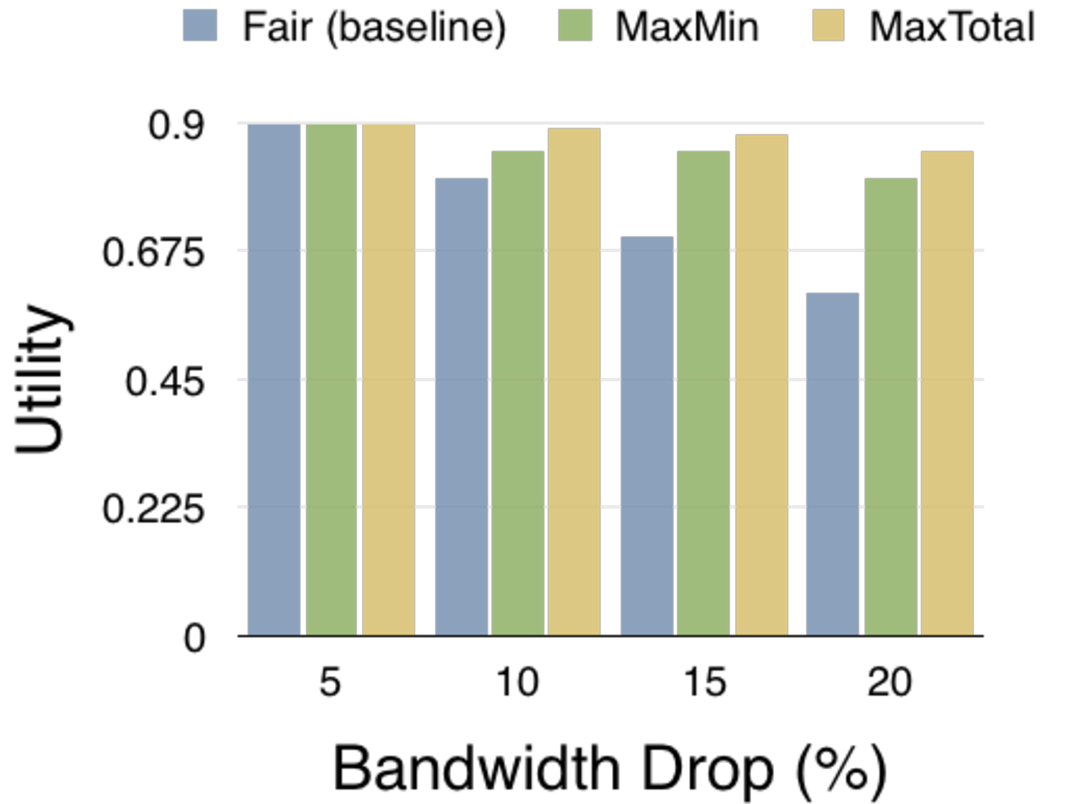
\includegraphics[width=\columnwidth]{figures/multitask.pdf}
  \caption{Multitask Scheduling}
  \label{fig:multitask}
\end{figure}

%%% Local Variables:
%%% mode: latex
%%% TeX-master: "sosp17"
%%% End:
